% \documentclass{beamer}
% \usetheme{Boadilla}

% \usepackage[english,greek]{babel}
% % \usepackage[greek,english]{babel}
% \usepackage[utf8]{inputenc}

% \newcommand{\tl}{\textlatin}
% \newcommand{\en}{\selectlanguage{english}}
% \newcommand{\gr}{\selectlanguage{greek}}


% \begin{document}

\section{Εισαγωγή}

\begin{frame}
  \frametitle{Περιγραφή προβλήματος}
  Το πρόβλημα της αναγνώρισης και εντοπισμού ανθρώπινης δράσης σε βίντεο έχει δύο κύριους στόχους:
  \begin{itemize}[(I)]
  \item<2-> Την αυτόματη αναγνώριση και ταξινόμησή οποιασδήποτε ανθρώπινης δραστηριότητας στο βίντεο.
  \item<3-> Τον αυτόματο εντοπισμό αυτής της δράσης στο βίντεο
  \end{itemize}

\end{frame}

\begin{frame}
  \frametitle{Προκλήσεις και \tl{Datasets}}
  \begin{figure}
    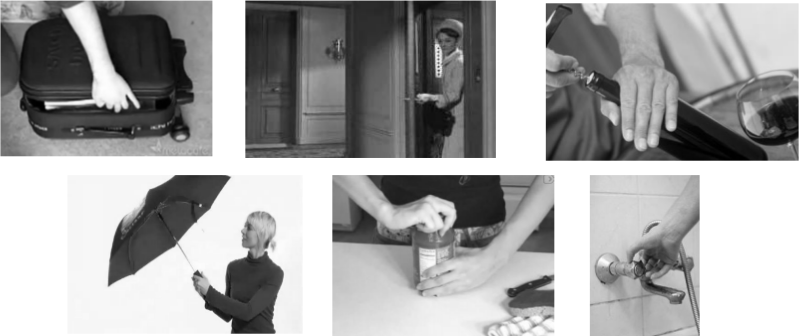
\includegraphics[scale=0.2]{open_example}
  \end{figure}
  \pause
  Παραδείγματα της δράσης «Ανοίγω»

\end{frame}




% \subsection{Applications}
% \subsection{Challenges and Datasets}
% \subsection{Motivation and Contributions}
% \end{document}